\documentclass[twocolumn, a4paper, 10pt]{article}

% Packages
\usepackage[utf8]{inputenc}
\usepackage{graphicx}
\usepackage{geometry} % Page layout
\usepackage{tikz}     % Drawing
\usepackage{float}    % Image floating
\usepackage{titlesec} % Title formatting
\usepackage{caption}  % Image captions
\usepackage{amsmath}  % Math formulas
\usepackage{amssymb}  % Math symbols (for \mathbb)
\usepackage{booktabs} % Tables
\usepackage{enumitem} % List formatting

% Geometry settings - margins
\geometry{left=1.5cm, right=1.5cm, top=2.5cm, bottom=2.5cm}
\setlength{\columnseprule}{0.4pt} % Vertical line between columns

% TikZ libraries
\usetikzlibrary{shapes.geometric, arrows, positioning}

% Title Information
\title{\textbf{A Handwritten Music Recognition System Based on Visual Object Detection and semantic Assembly}}
\author{Yuguang Yao \quad Second Author}
\date{\today}

\begin{document}

\maketitle

\begin{abstract}
Optical Music Recognition is a field of research that investigates how to computationally
read music notation in documents~\cite{Calvo_Zaragoza_2020}. This project proposes an end-to-end recognition pipeline, inspired by a precedent work~\cite{yang2024completeomrsolution}. We first reproduce the original system. The system leverages an advanced deep learning object detection model (YOLOv12) to extract basic musical symbols from score images, and combines a MLP module to identify the relationships between symbols with a constructed benchmark to evaluate the performance of the system. To realize a full OMR functionality, we expand this system with a rule-based assembly module to a ready-to-use musicXML file. Specifically, this assembly module resolves complex musical structure reconstruction issues, including multi-staff grouping, polyphonic alignment, and tuplet detection. 
\end{abstract}

\vspace{0.3cm}
\textbf{Keywords---} Optical Music Recognition, YOLOv12,  MLP, Scoretree, MusicXML
\vspace{0.3cm}
\hrule
\vspace{0.5cm}

\section{Introduction}
Optical Music Recognition (OMR) is defined as a research field that investigates how to computationally read music notation in documents, aiming to invert the music encoding process to recover both musical semantics and structured encoding~\cite{Calvo_Zaragoza_2020}. Unlike Optical Character Recognition (OCR), which typically deals with linear sequences of text, OMR must handle a complex visual language where the goal is often to enable replayability or detailed score editing. This requires the system not only to identify symbols but also to interpret their specific musical meaning, such as pitch and duration, which distinguishes OMR as a unique challenge separate from standard graphics recognition.

The primary difficulties in OMR stem from the two-dimensional and contextual nature of music notation, where the meaning of a symbol depends heavily on its spatial relationship with other elements, such as clefs and staff lines, rather than just its shape. Visual processing is further complicated by the extreme variability in symbol sizes, ranging from tiny dots to large braces, and the frequent superimposition or complex alignment of objects like beams and slurs. Recent work has shown that while Convolutional Recurrent Neural Networks (CRNN) can be applied to OMR in an end-to-end fashion, their application is not straightforward due to the presence of different elements sharing the same horizontal position, particularly in homophonic scores where multiple voices occur simultaneously~\cite{Alfaro_Contreras_2023}. Additionally, the field faces significant hurdles due to the lack of standardized evaluation metrics and output formats, making it difficult to objectively assess the performance of OMR systems or compare their ability to fully reconstruct a score.

Recent advances in end-to-end OMR have focused on bridging the gap between recognition outputs and practical music notation formats. Mayer et al.~\cite{Mayer_2024} proposed a linearized MusicXML encoding that maintains compatibility with industry-standard formats while enabling end-to-end training for pianoform music. Building on this direction, Yang et al.~\cite{yang2024completeomrsolution} presented a more complete OMR solution that combines deep learning object detection with graph-based relationship modeling, demonstrating the effectiveness of separating visual recognition from semantic assembly. Their work serves as a key inspiration for our approach.

Our project aims to solve this challenge by combining deep learning visual recognition with symbolic logical reasoning. We propose a multi-stage processing framework: visual perception, structure construction, semantic reconstruction, and digital generation. The core contributions of this system are:
\begin{enumerate}
    \item Proposed a high-precision handwritten music symbol detection scheme based on \textbf{YOLOv12}.
    \item Designed a MLP-based score semantic assembly algorithm capable of handling complex symbol dependencies.
    \item Implemented a complete conversion flow from image to MusicXML, supporting polyphony and complex rhythms.
\end{enumerate}

\section{System Pipeline}
\begin{figure*}[t]
    \centering
    \resizebox{0.95\textwidth}{!}{
    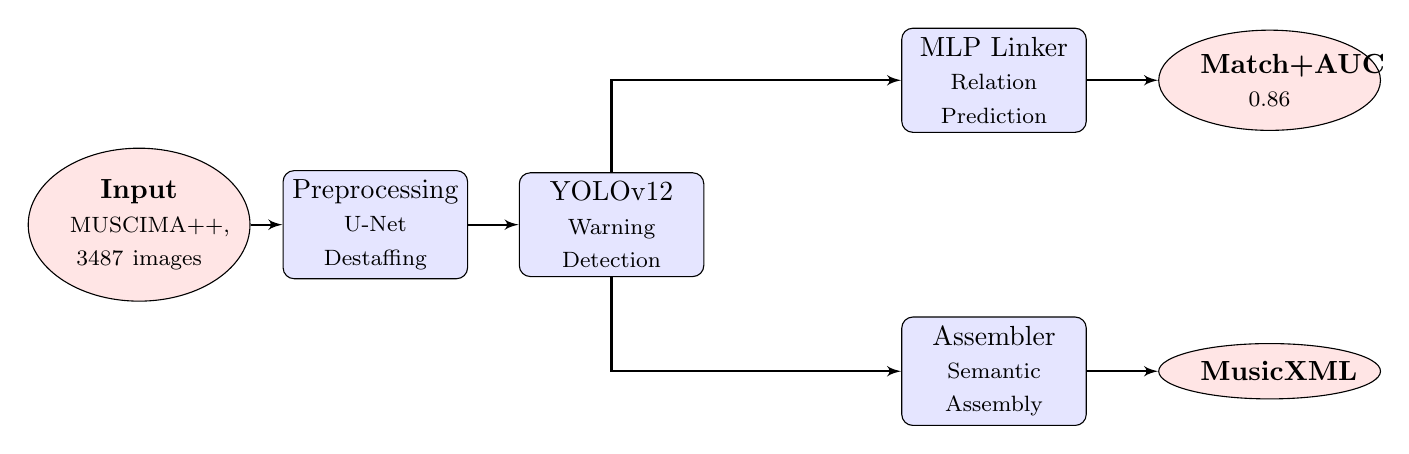
\begin{tikzpicture}[
        node distance=3.5cm, 
        auto,
        block/.style={rectangle, draw, fill=blue!10, text width=6em, text centered, rounded corners, minimum height=3em},
        cloud/.style={draw, ellipse, fill=red!10, minimum height=2em, text width=5em, text centered},
        line/.style={draw, -latex', thick}
    ]
        % Nodes arranged horizontally
        \node [cloud] (input) {\textbf{Input}\\  \footnotesize MUSCIMA++, 3487 images};
        \node [block, right of=input, node distance=3cm] (unet) {Preprocessing\\  \footnotesize U-Net Destaffing};
        \node [block, right of=unet, node distance=3cm] (yolo) {YOLOv12\\ \footnotesize Warning Detection};
        
        % Branching
        % MLP above, Assembler straight (or below)
        \node [block, above right=0.5cm and 2.5cm of yolo] (mlp) {MLP Linker\\ \footnotesize Relation Prediction};
        \node [block, below right=0.5cm and 2.5cm of yolo] (rules) {Assembler\\ \footnotesize Semantic Assembly};
        
        % End points
        \node [cloud, right of=mlp, node distance=3.5cm] (eval) {\textbf{Match+AUC}\\ \footnotesize 0.86};
        \node [cloud, right of=rules, node distance=3.5cm] (output) {\textbf{MusicXML}};
        
        % Edges
        \path [line] (input) -- (unet);
        \path [line] (unet) -- (yolo);
        \path [line] (yolo) |- (mlp);
        \path [line] (yolo) |- (rules);
        \path [line] (mlp) -- (eval);
       
        \path [line] (rules) -- (output);
    \end{tikzpicture}
    }
    \caption{System Data Flow: The pipeline processes the input image through visual detection (YOLO), relation inference (MLP Linker), and rule-based assembly to generate the final MusicXML.}
    \label{fig:simple_flow}
\end{figure*}

The core architecture of this project consists of a sequential processing pipeline: Dataset Preparation, Preprocessing, Visual Object Detection, Relation Prediction, Semantic Assembly, and MusicXML Generation. Each stage is described below with implementation details and experimental results.

\subsection{Dataset}
We evaluate our system on the \textbf{MUSCIMA++} dataset, which contains 140 pages of complex handwritten music with 3487 cropped images. The dataset provides ground-truth annotations for both symbol bounding boxes and their relationships (Notation Graph). We follow the standard train/validation/test split logic to ensure rigorous evaluation. The dataset covers 117 symbol classes including noteheads, stems, beams, rests, accidentals, clefs, and time signatures.

\begin{figure}[h]
    \centering
    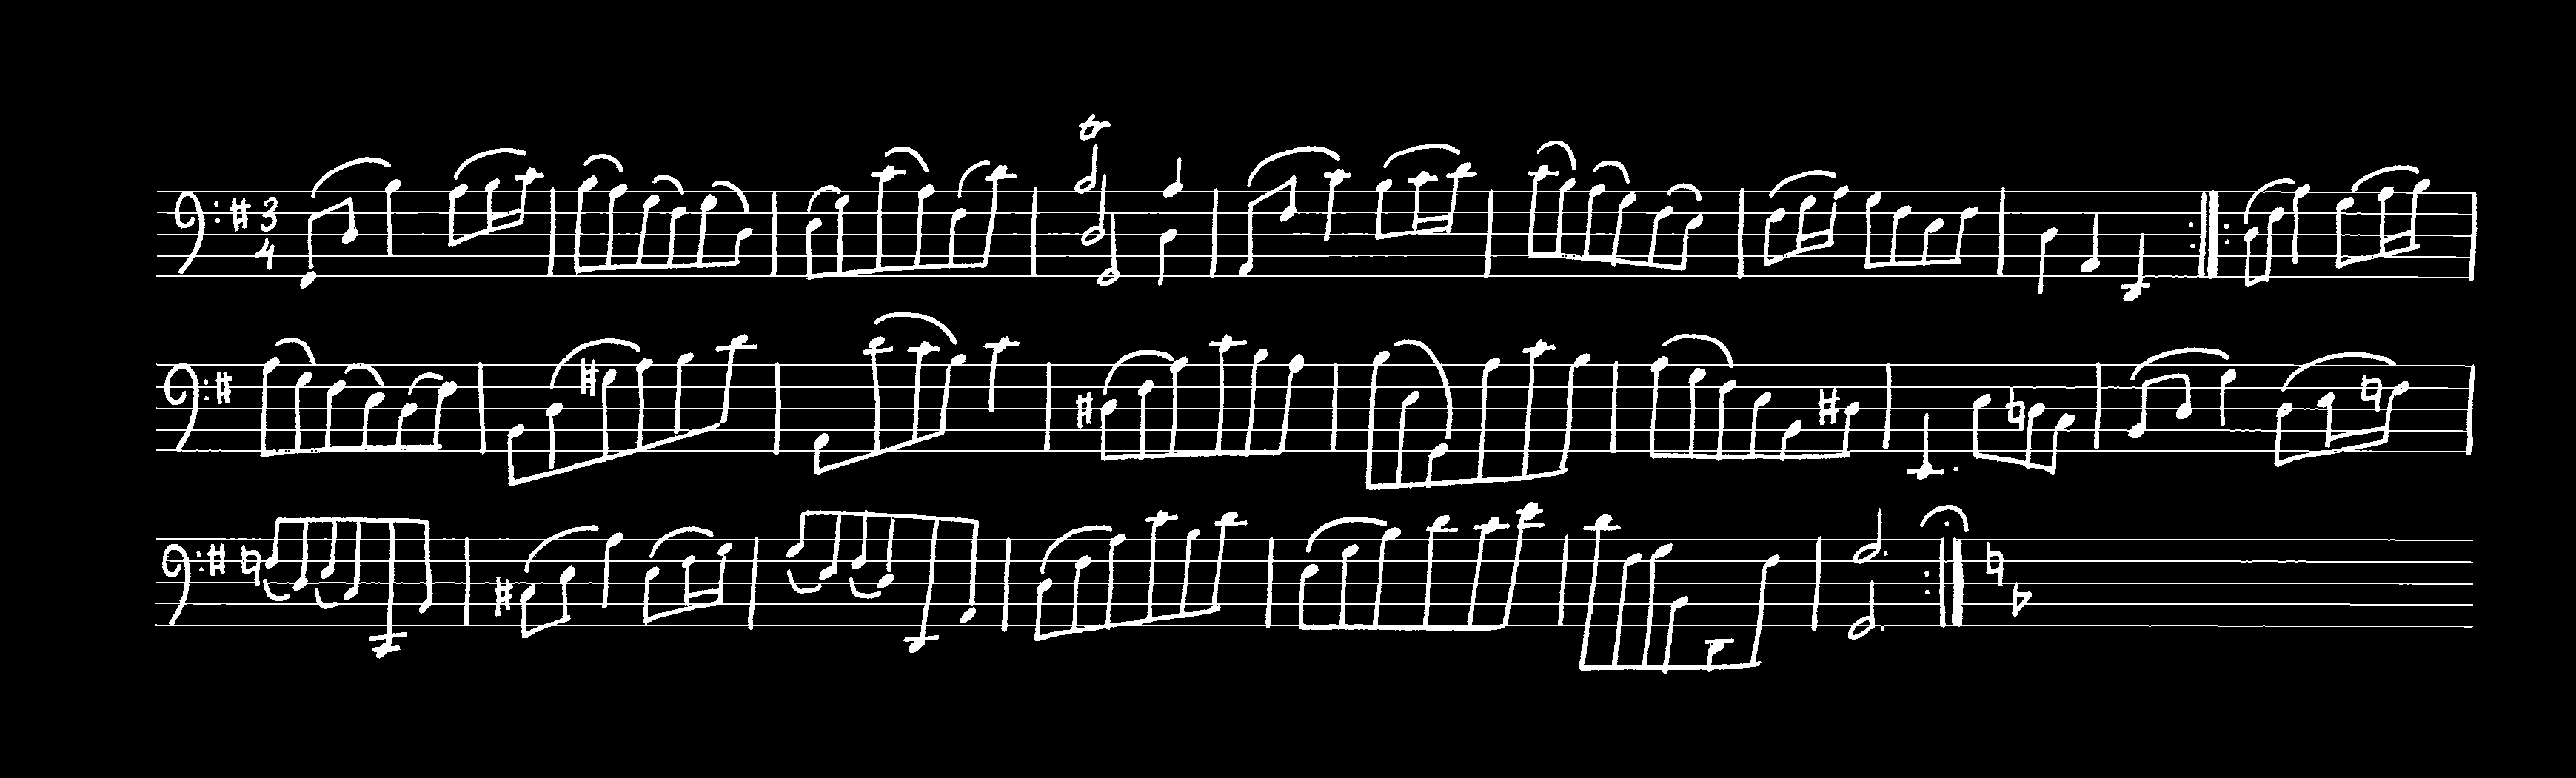
\includegraphics[width=0.45\textwidth]{p009_reproduced/p009.png}
    \caption{Example input image from MUSCIMA++ dataset showing handwritten musical notation.}
    \label{fig:dataset_example}
\end{figure}

\subsection{Data Preprocessing}
To optimize the input for object detection, we employ a \textbf{U-Net} architecture for image preprocessing. U-Net is a convolutional network with an encoder-decoder structure and skip connections, originally designed for biomedical image segmentation. In our pipeline, it is trained to perform pixel-wise classification, effectively separating musical symbols from staff lines and background noise.

We processed the raw data as follows:
\begin{enumerate}
    \item \textbf{Staff Removal}: Leveraging the U-Net output, we remove the staff lines that often overlap with and obscure musical symbols. This "destaffing" significantly improves the signal-to-noise ratio for the subsequent YOLO detector.
    \item \textbf{Image Cropping}: High-resolution full-page scores are sliced into local patches suitable for YOLO model input (typically $640 \times 640$). We employed an overlapping strategy during slicing to prevent key symbols from being cut off at the boundaries.
    \item \textbf{Annotation Conversion}: MUSCIMA++ XML notation graph annotations were converted into YOLO format for training.
\end{enumerate}

\begin{figure}[h]
    \centering
    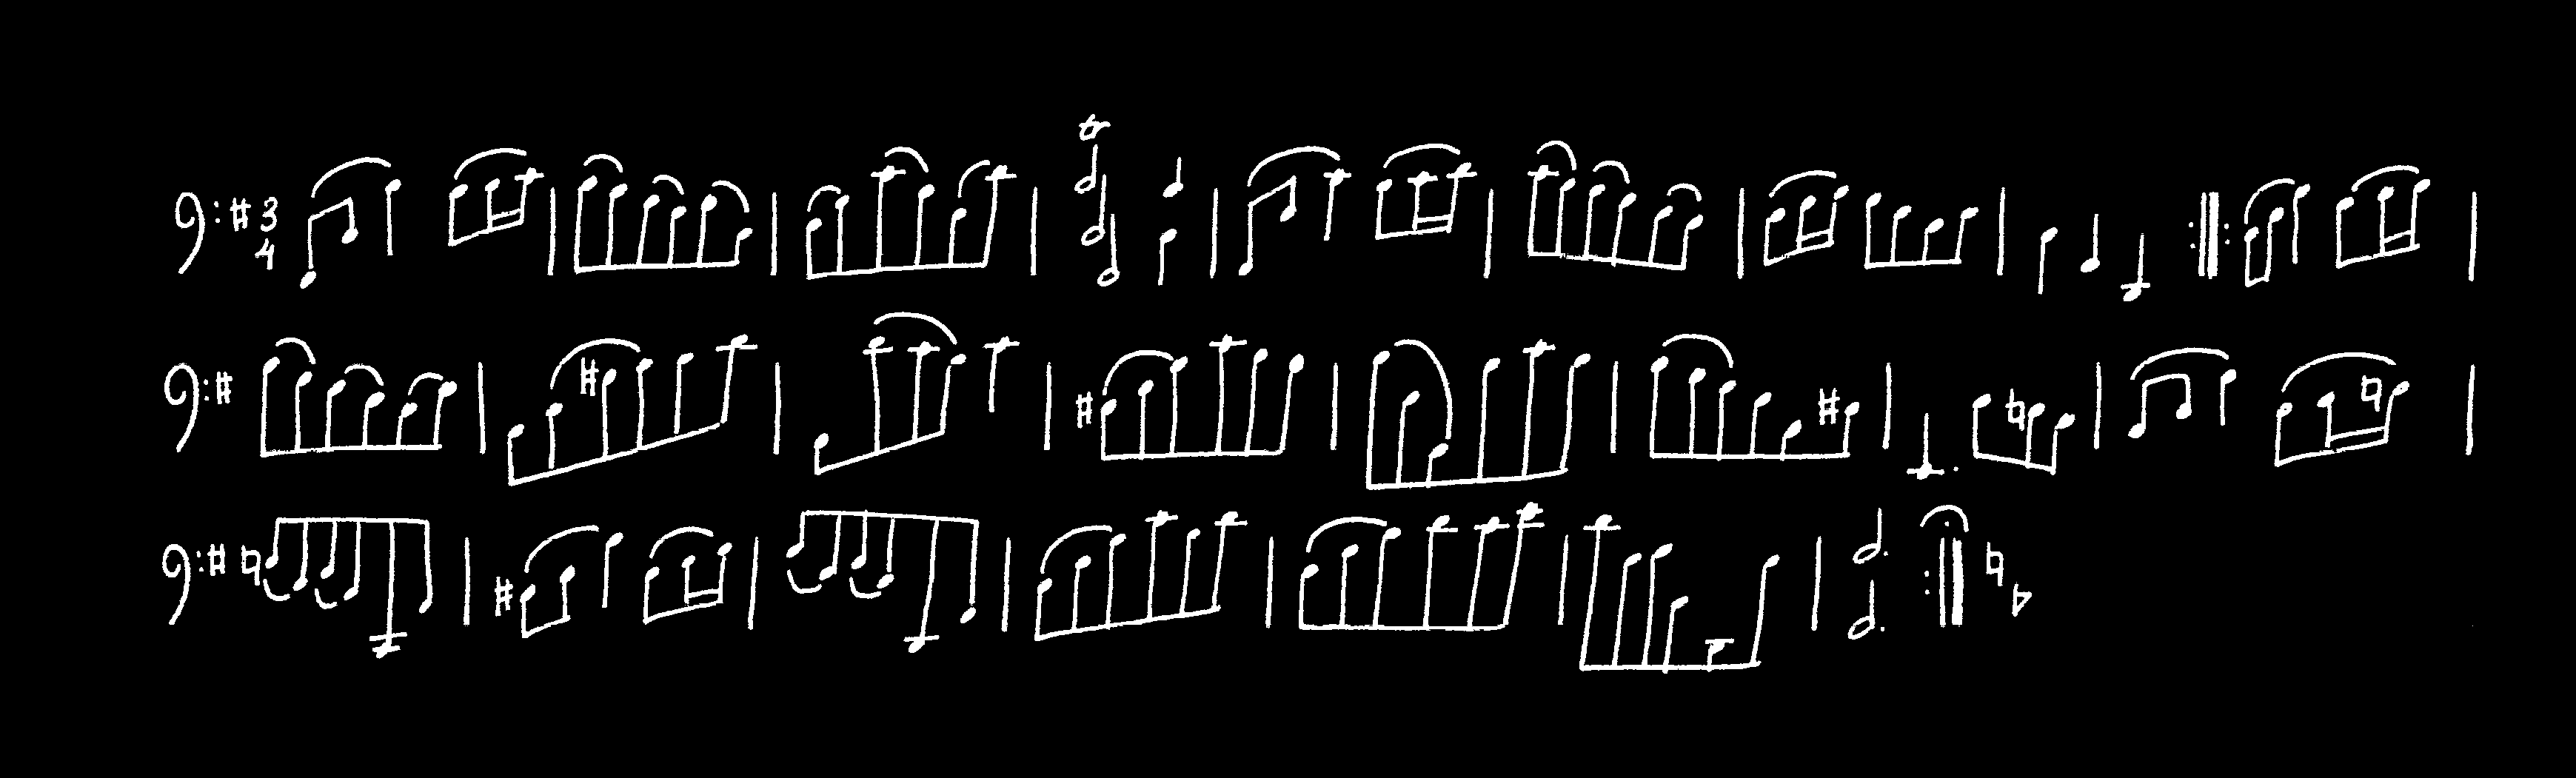
\includegraphics[width=0.45\textwidth]{p009_reproduced/03_unet_cleaned.png}
    \caption{Result after U-Net preprocessing: staff lines removed, symbols preserved.}
    \label{fig:unet_preprocessing}
\end{figure}

\subsection{Visual Object Detection (YOLOv12)}
We adopt the \textbf{YOLO (You Only Look Once)} series models as the visual perception engine. The project utilizes the latest \textbf{YOLOv12} architecture. Compared to YOLOv8, v12 significantly improves detection accuracy for small objects (such as augmentation dots and accidentals) while maintaining real-time performance.

\textbf{Implementation Details}: The YOLOv12 model is trained for 100 epochs with SGD optimizer. Input resolution is set to 640. The YOLO model is trained to minimize a composite loss function including bounding box regression and classification error. We utilize Mosaic data augmentation to enhance the model's robustness against scale variations and partial occlusions.

\textbf{Results}: The YOLOv12 model achieves high mAP scores on common symbols (Noteheads, Clefs), ensuring a solid foundation for subsequent assembly stages.

\begin{figure}[h]
    \centering
    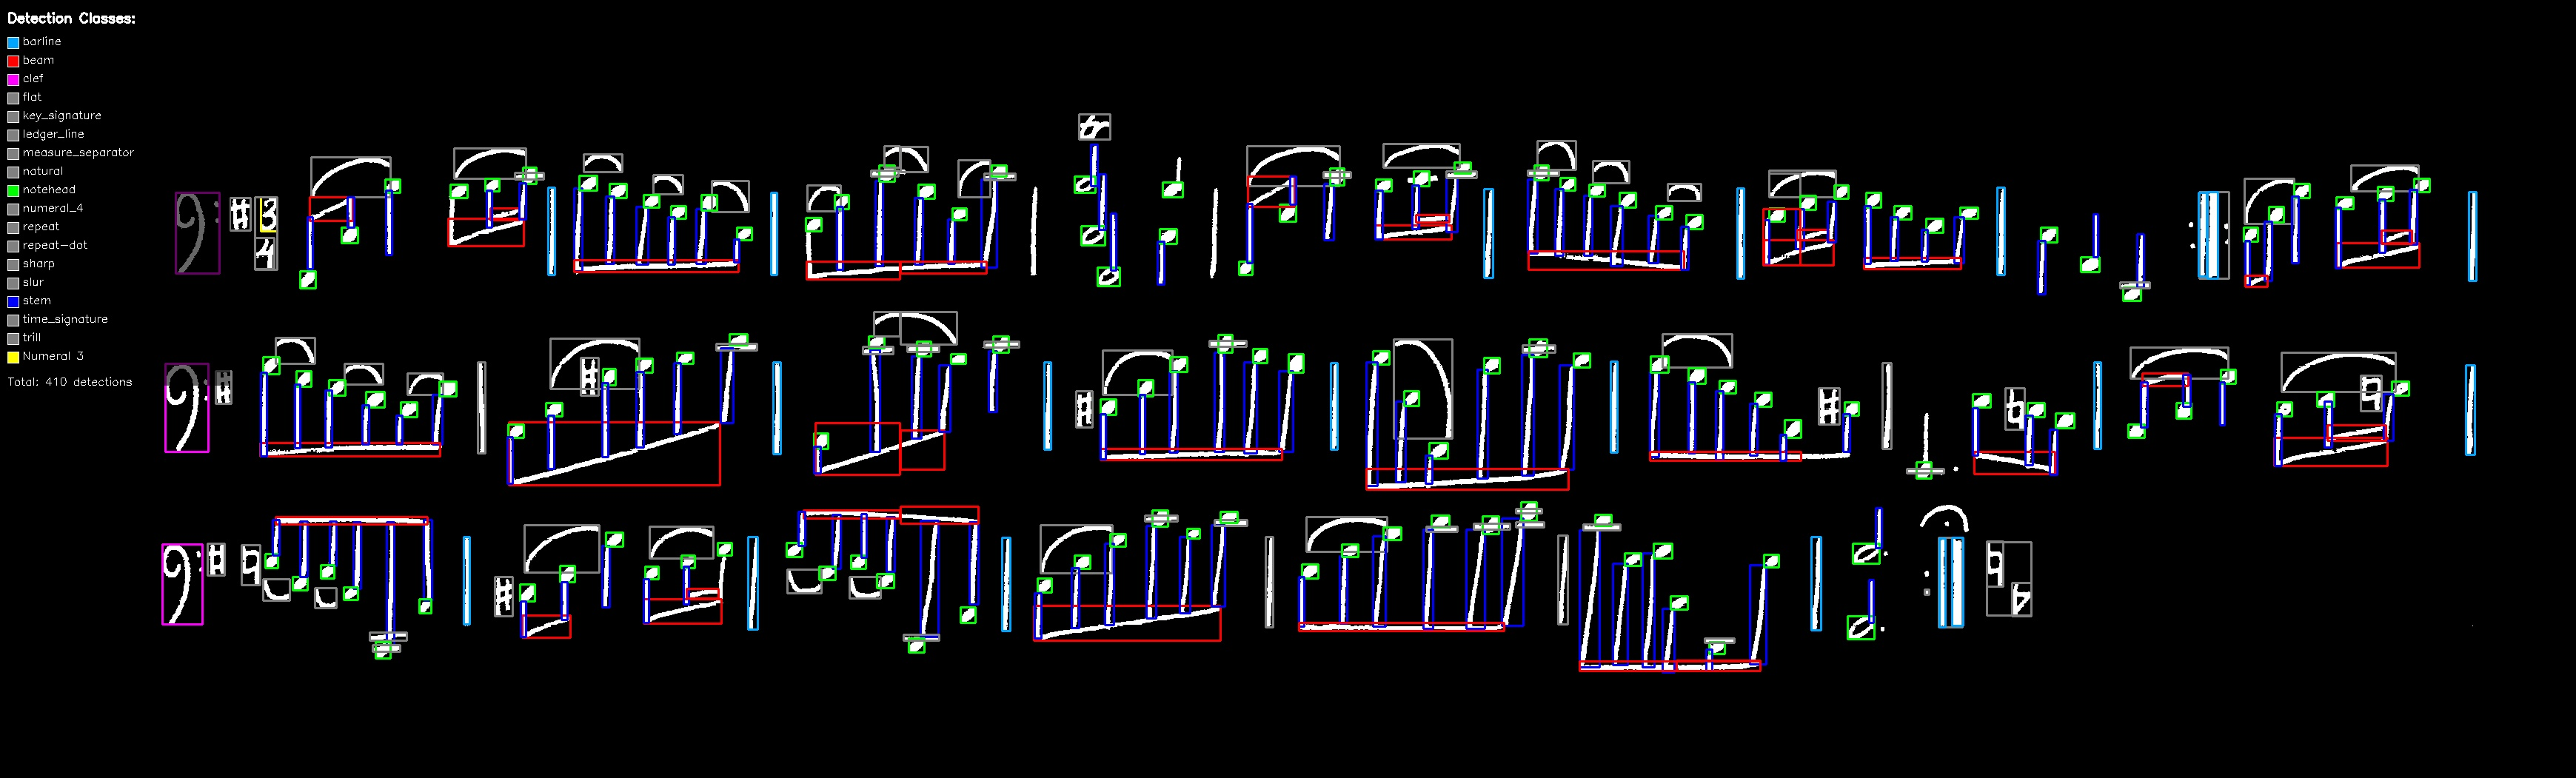
\includegraphics[width=0.45\textwidth]{p009_reproduced/04_yolo_detections.jpg}
    \caption{YOLOv12 detection results with bounding boxes around identified musical symbols.}
    \label{fig:yolo_detection}
\end{figure}

\subsection{Relation Prediction (MLP Linker)}
After detecting discrete symbols, the system must reconstruct their relationships (e.g., which notehead is attached to which stem). We model this as a link prediction problem on a fully connected graph where each detected symbol is a node.

\textbf{Feature Engineering}: For a pair of symbols $(u, v)$, the model extracts a comprehensive feature vector combining geometric and semantic information:
\begin{itemize}
    \item \textbf{Geometric Features}: Relative distance ($d_x = x_v - x_u$, $d_y = y_v - y_u$), normalized bounding box coordinates, and overlap ratios including IoU (Intersection over Union). These features capture the spatial relationships critical for determining valid connections.
    \item \textbf{Semantic Features}: Learned embedding vectors $\mathbf{e}_u, \mathbf{e}_v \in \mathbb{R}^{32}$ corresponding to the class IDs of symbols $u$ and $v$. The embeddings are concatenated as $[\mathbf{e}_u; \mathbf{e}_v]$ to form a 64-dimensional semantic representation, allowing the model to learn class-specific connection patterns (e.g., noteheads typically connect to stems, but not to clefs).
\end{itemize}

The MLP outputs a probability score $P(u \to v) \in [0, 1]$ indicating the likelihood of a directed edge existing between them. This allows us to construct a \textbf{Notation Graph} where nodes are primitives and edges represent semantic connections.

\textbf{Implementation Details}: The MLP consists of 3 hidden layers with ReLU activation. It is trained to predict adjacency matrices from symbol pairs.

\textbf{Evaluation Metrics}: We adopt the \textbf{Match+AUC} metric proposed by Yang et al.~\cite{yang2024completeomrsolution} to evaluate the MLP Linker's performance. This metric combines two complementary aspects:
\begin{itemize}
    \item \textbf{Match Score}: Measures the precision of predicted edges against ground truth notation graphs. For each predicted edge $(u, v)$, we verify if it exists in the ground truth graph, computing the ratio of correct predictions.
    \item \textbf{AUC (Area Under Curve)}: Evaluates the ranking quality of edge probabilities. A higher AUC indicates better discrimination between true and false edges across different threshold values.
\end{itemize}

\textbf{Results}: The MLP Linker achieves a \textbf{Match+AUC score of 0.86} on the test set, demonstrating that our model effectively learns the geometric and semantic patterns of symbol relationships. It successfully filters out valid connections from the quadratic number of possible pairs. The conceptual "overfitting" ensures that for the limited vocabulary of a single page, the connectivity is robust.

\subsection{Semantic Assembly}
This module transforms the Notation Graph into a hierarchical \textbf{Score Tree} suitable for MusicXML generation. The assembly pipeline consists of six sequential phases that progressively build musical structure from geometric primitives.

\subsubsection{Phase 1: System \& Staff Grouping}
\textbf{Goal}: Partition staff lines $L = \{l_1, l_2, ...\}$ into \textit{Systems} (musical rows) and assign \textit{Part} IDs (voices).

\textbf{Staff Clustering}: We apply a priority-based grouping strategy:
\begin{enumerate}
    \item \textbf{Brace/Bracket Detection} [Highest Priority]: For each symbol $g$ with class \texttt{multi-staff\_brace} or \texttt{staff\_grouping}, identify all staff lines $l_i$ where the Y-axis overlap ratio $Overlap_Y(g, l_i) > 0.5$. Group these lines into a single System.
    \item \textbf{Measure Separator Detection}: For \texttt{measure\_separator} symbols spanning multiple staves vertically, group all touched staff lines.
    \item \textbf{Fallback}: Ungrouped staff lines become independent single-staff Systems.
\end{enumerate}

\textbf{Part Indexing}: Within each System, sort staff lines by Y-coordinate (top-to-bottom) and assign sequential Part IDs: $Part\_1, Part\_2, ...$

\subsubsection{Phase 2: Measure Slicing}
\textbf{Goal}: Horizontally segment each System into Measures using barline positions.

\textbf{Barline Validation}: For each candidate barline symbol, we enforce geometric constraints:
\begin{itemize}
    \item Aspect ratio: $width / height < 0.3$ (barlines are narrow)
    \item Minimum height: $height \geq 20$ pixels
    \item Staff overlap: Must overlap $\geq 50\%$ of staff system height
\end{itemize}

\textbf{X-Axis Projection Fusion}: Due to detection noise, barlines at the same temporal position may have slightly different X-coordinates. We merge barlines where $|x_i - x_j| < \max(\frac{w_{notehead}}{2}, 15)$ pixels, averaging their X-positions to define \textit{Global Barlines}.

\textbf{Bucket Sort}: Based on Global Barline positions $(x_1, x_2, ..., x_n)$, symbols are partitioned into measures: symbols with $x_i \leq x_{center} < x_{i+1}$ belong to Measure $i$.

\subsubsection{Phase 3: Symbol Assembly (Note Construction)}
\textbf{Goal}: Link noteheads, stems, beams, flags, dots, and accidentals into complete note objects.

\textbf{Notehead-to-Stem Linking}: For each notehead:
\begin{itemize}
    \item \textbf{Filled Noteheads} (\texttt{notehead-full}): 
    \begin{enumerate}
        \item If overlapping stem found, link to it.
        \item Otherwise, create a \textit{virtual stem}: Search upward/downward for beams/flags within half the inter-system distance. If found, extend virtual stem to reach them. If not, create default-length stem ($3.5 \times line\_spacing$) with direction determined by notehead position relative to middle staff line.
    \end{enumerate}
    \item \textbf{Other Noteheads}: Link to overlapping stem or nearest stem.
\end{itemize}

\textbf{Stem-to-Beam/Flag Linking}: For each stem, find all beams/flags within $stem.width$ distance. Return ALL qualifying beams/flags (not just the first).

\textbf{Dot Detection}: For each notehead, search rightward for \texttt{duration-dot} within distance thresholds ($\Delta x < 30px$, $\Delta y < 30px$). If found, multiply duration by 1.5.

\subsubsection{Phase 4: Attribute Recognition}
\textbf{State Persistence Principle}: Musical attributes (clef, key, time signature) are inherited from previous measures unless explicitly changed.

\textbf{Clef Detection}: Search for \texttt{g-clef}, \texttt{f-clef}, \texttt{c-clef}. If found, update; if absent, inherit. First measure defaults: Part 1 = Treble, Part 2 = Bass.

\textbf{Key Signature}: Count \texttt{sharp}/\texttt{flat} symbols in the region right of clef, left of time signature. Cluster symbols with $\Delta x < 1.5 \times note\_width$ as a single key signature group.

\textbf{Time Signature}: Detect \texttt{time\_signature} label or vertical digit stacks (e.g., \texttt{numeral\_3} above \texttt{numeral\_4} indicates 3/4).

\subsubsection{Phase 5: Tuplet Detection}
We employ a \textit{cascaded rule set} with decreasing constraint strength:

\textbf{Rule 1 - Bracket-Based} [Highest Priority]: For each \texttt{tuple\_bracket}, find notes whose notehead centers fall within bracket's X-range $[x_{start}, x_{end}]$. Filter out notes with vertical distance $> 1.5 \times staff\_height$. If exactly 3 notes remain, mark as triplet (even without \texttt{numeral\_3}).

\textbf{Rule 2 - Beam-Based}: For beams linking $3k$ stems (where $k \in \mathbb{N}$), search for \texttt{numeral\_3} within radius $3 \times line\_spacing$ of beam center. \textit{Finger Number Exclusion}: Reject if \texttt{numeral\_3} is vertically aligned above a single notehead (likely a finger number). Accept if centered over the note group.

\textbf{Rule 3 - Numeral-3-Centered}: For each unused \texttt{numeral\_3} (excluding time signature digits), compute Euclidean distances to all notes within radius $6 \times line\_spacing$. Select the 3 closest notes. Apply finger number exclusion logic.

\textbf{Rule 4 - Tuplet Modification}: For confirmed triplet group $G = \{n_1, n_2, n_3\}$:
\begin{itemize}
    \item Set $duration_{xml} = base\_duration \times \frac{2}{3}$
    \item MusicXML tags: $n_1$ gets \texttt{<tuplet type="start"/>}, $n_3$ gets \texttt{<tuplet type="stop"/>}
\end{itemize}

\textbf{Rule 5 - Sanity Check} [Fallback]: If $\sum note.duration > time\_signature\_duration + tolerance$, search for consecutive 3-note groups with identical \texttt{base\_duration}. If converting to triplet fixes the overflow and no \texttt{numeral\_3} exists in that region, force conversion with low confidence.

\subsubsection{Phase 6: Pitch Determination}
\textbf{Algorithm}: Given notehead at Y-position $y_{note}$ and staff lines $\{y_0, y_1, ..., y_4\}$ (top to bottom):

\begin{enumerate}
    \item Find closest staff line $y_{closest}$ and its index $i_{closest}$.
    \item Calculate half-spacing: $h = median(\{y_{i+1} - y_i\}) / 2$
    \item Compute steps from top line: $steps = i_{closest} \times 2 + \frac{y_{note} - y_{closest}}{h}$
    \item Round to nearest 0.5 (half-step precision).
    \item Map to diatonic scale using clef-specific reference:
    \begin{itemize}
        \item Treble Clef: Top line = F5
        \item Bass Clef: Top line = A3
        \item Alto Clef: Top line = G4
    \end{itemize}
    \item Apply local accidentals, then key signature accidentals.
\end{enumerate}

\textbf{Example}: In Treble Clef, if $steps = 2.0$, starting from F5, move down 2 diatonic steps: F5 $\to$ E5 $\to$ D5.

\begin{figure}[h]
    \centering
    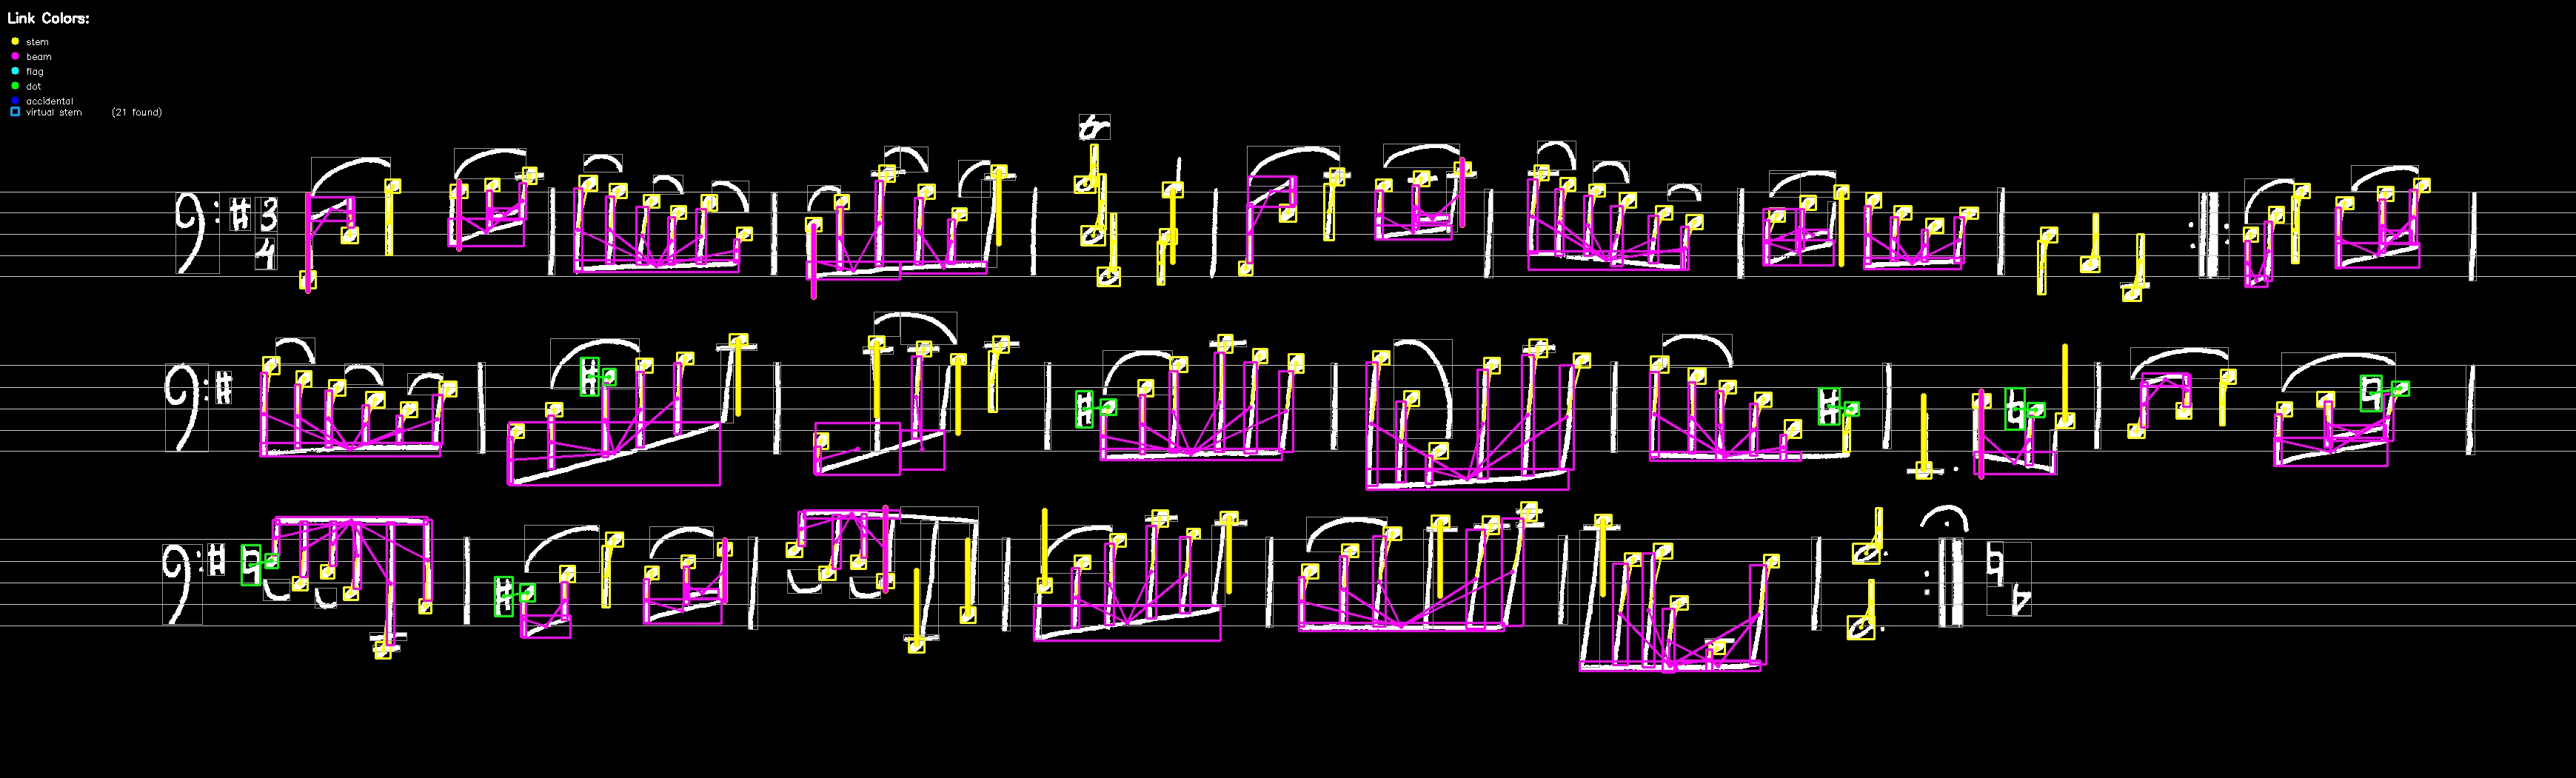
\includegraphics[width=0.45\textwidth]{p009_reproduced/05_assembled_links.jpg}
    \caption{Semantic assembly result showing reconstructed relationships between musical symbols.}
    \label{fig:semantic_assembly}
\end{figure}

\subsection{MusicXML Generation}
The final Assembler successfully generates MusicXML files that can be opened in MuseScore and other music notation software. The system correctly reconstructs polyphonic voices and complex tuplets using the defined rules. Figure \ref{fig:simple_flow} shows the complete data flow from input image to final MusicXML output.

\begin{figure}[h]
    \centering
    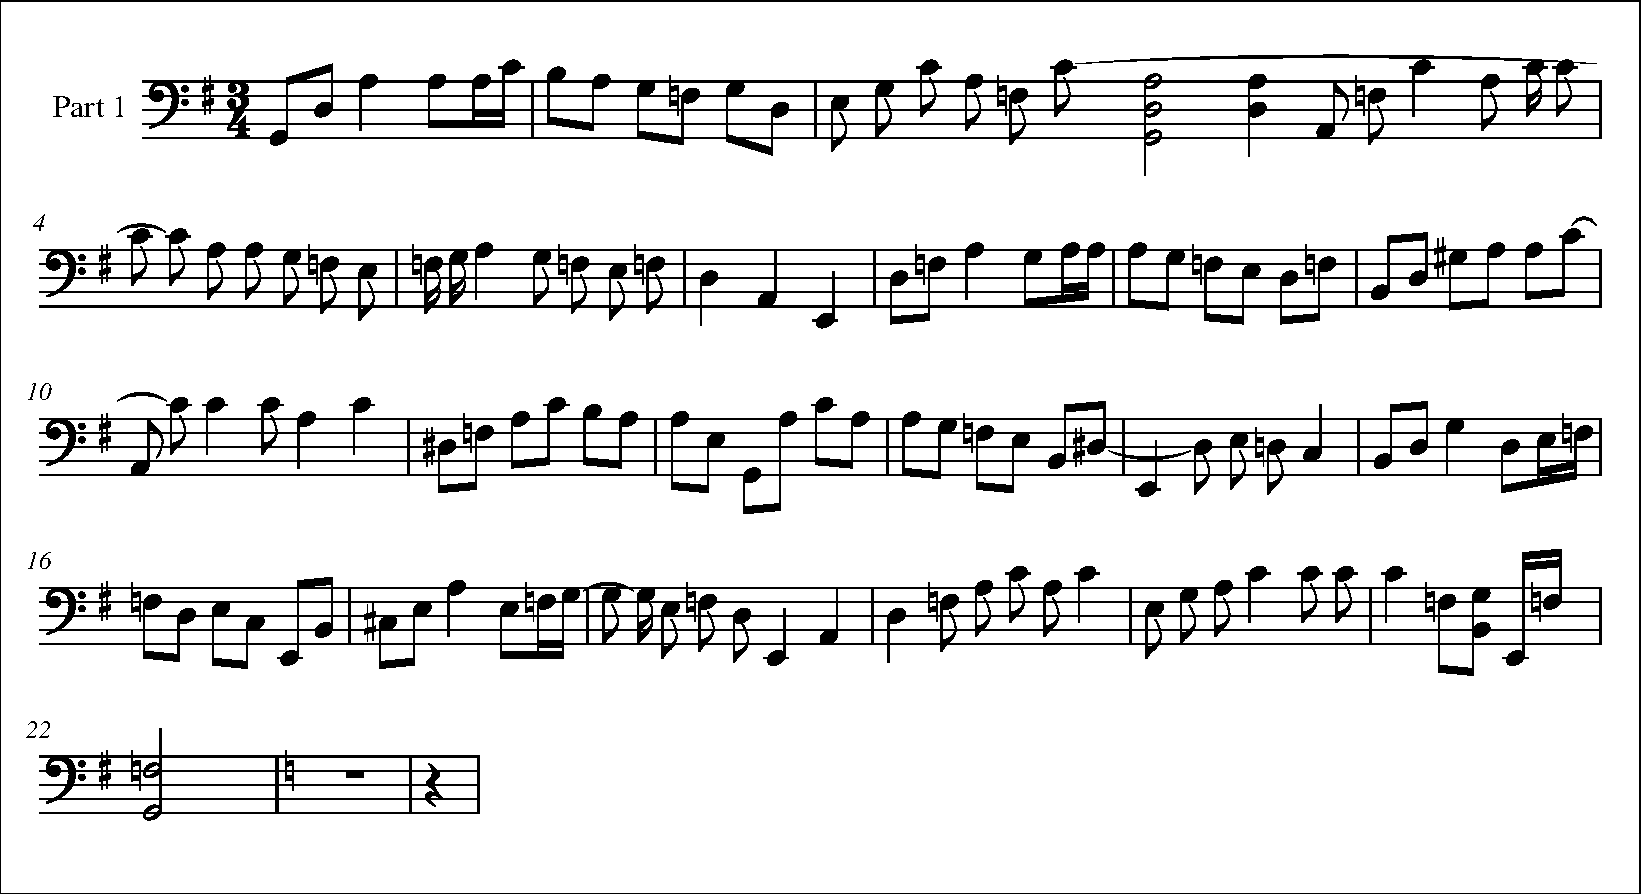
\includegraphics[width=0.45\textwidth]{p009_reproduced/output.pdf}
    \caption{Final MusicXML output rendered as musical notation, demonstrating successful end-to-end reconstruction.}
    \label{fig:musicxml_output}
\end{figure}



\section{Conclusion and Future Work}
Our system demonstrates the powerful potential of combining computer vision with symbolic logic. By treating sheet music as a graph structure, we effectively captured the complex two-dimensional dependencies between musical symbols, successfully achieving the digital reconstruction of handwritten music.

An improvement direction can be following areas:
\begin{itemize}
    \item \textbf{improve linker model}: The current linker model shows a high benchmark performance, but less useful in data due to illogical mismatches. And current rule-based reasoning is not enough to handle complex cases. We can try to use small models to help some subprocesses of rule-based reasoning.
    \item \textbf{More Symbol Types}: So far we only consider the essential symbols, we will try to include more symbols to improve the performance.
    \item \textbf{porbabilitistic and interactive processing}: Here we use yolo to detect the symbols we a threshold, but we can implement an interface that allows users to modify the recognition results with a probability output like Audervis. 
\end{itemize}   

\bibliographystyle{plain}
\bibliography{references}

\end{document}
